\chapter{Diseño}

{\color{blue}


Se van a mostrar las tecnologías usadas en el proyecto, así como las decisiones tomadas a la hora del desarrollo del software. En este proyecto, tenemos por un lado nuestra aplicación, la cual va a recoger todos los datos y por otro lado tenemos un dispositivo, que este es una Raspberry PI \cite{raspberry-specs}, prestada por mis tutores de proyecto. Para hacer la conexión entre aplicación y dispositivo se necesita hacer uso de un protocolo de mensajería, en este caso se opta por el uso de MQTT. \\

También se va a mostrar como se va a proceder para la explotación de la vulnerabilidad y cuestiones a tener en cuenta.

\section{Tecnologías usadas en la creación de la aplicación}

\subsection{Lenguaje de programación}

Se ha optado por usar Python, fue creado a principios de los años 90 por Guido van Rossum en el Stichting Mathematisch Centrum en los Países Bajos como sucesor de un lenguaje llamado ABC. Guido sigue siendo el principal autor de Python, aunque incluye muchas contribuciones de otras personas. \\

En mayo de 2000, Guido y el equipo de desarrollo del núcleo de Python se trasladaron a BeOpen.com para formar el equipo BeOpen PythonLabs. En octubre del mismo año, el equipo de PythonLabs se trasladó a Digital Creations. En 2001, se formó la Python Software Foundation, una organización sin ánimo de lucro creada específicamente para poseer la propiedad intelectual relacionada con Python. \cite{python-history} \\

Python es un lenguaje de alto nivel de programación interpretado cuya filosofía hace hincapié en la legibilidad de su código, se utiliza para desarrollar aplicaciones de todo tipo. Se trata de un lenguaje de programación multiparadigma, ya que soporta parcialmente la orientación a objetos, programación imperativa y, en menor medida, programación funcional. Es un lenguaje interpretado, dinámico y multiplataforma. \cite{python-wiki} \\

Para este proyecto es una buena opción ya que gracias a paquetes como \textbf{paho-mqtt}, que proporciona una clase cliente que permite a las aplicaciones conectarse a un broker MQTT para publicar mensajes, y para suscribirse a temas y recibir mensajes publicados, podemos hacer conexiones a mqtt de una manera muy sencilla. \cite{paho-mqtt}

\subsection{Pycharm}

PyCharm es un entorno de desarrollo integrado utilizado en programación informática, concretamente para el lenguaje de programación Python. Está desarrollado por la empresa checa JetBrains. Proporciona análisis de código, un depurador gráfico, un probador de unidades integrado, integración con sistemas de control de versiones (VCS), y soporta el desarrollo web con Django, así como la ciencia de datos con Anaconda. \\

PyCharm es multiplataforma, con versiones para Windows, macOS y Linux. La Community Edition (edición comunitaria) se publica bajo la Licencia apache, y también hay una Professional Edition (edición profesional) con características adicionales publicada bajo una licencia propietaria financiada por suscripción y también una versión educativa, que gracias a la universidad de Granada podemos hacer uso de esta licencia. \cite{pycharm}

\subsection{Diagrama de clases}

Para hacer la comunicación entre el dispositivo y la aplicación se propone el siguiente diagrama de clases que describe la estructura del sistema. 

\begin{figure}[p]
    \centering
    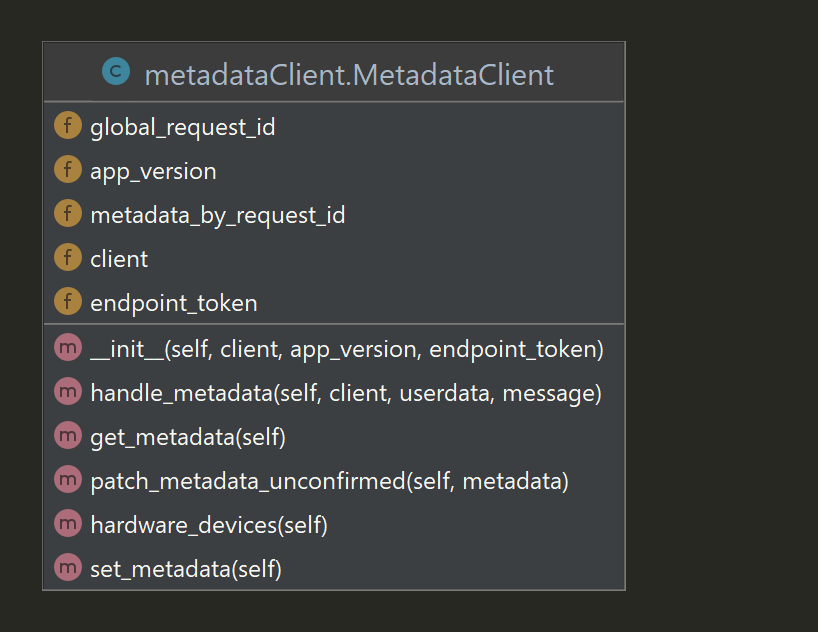
\includegraphics[width=\linewidth]{imagenes/metadataClient.png}
    \caption{Clase de envio de metadatos del dispositivo}
    \label{fig:figure-diseño1}
\end{figure}

\begin{figure}[p]
    \centering
    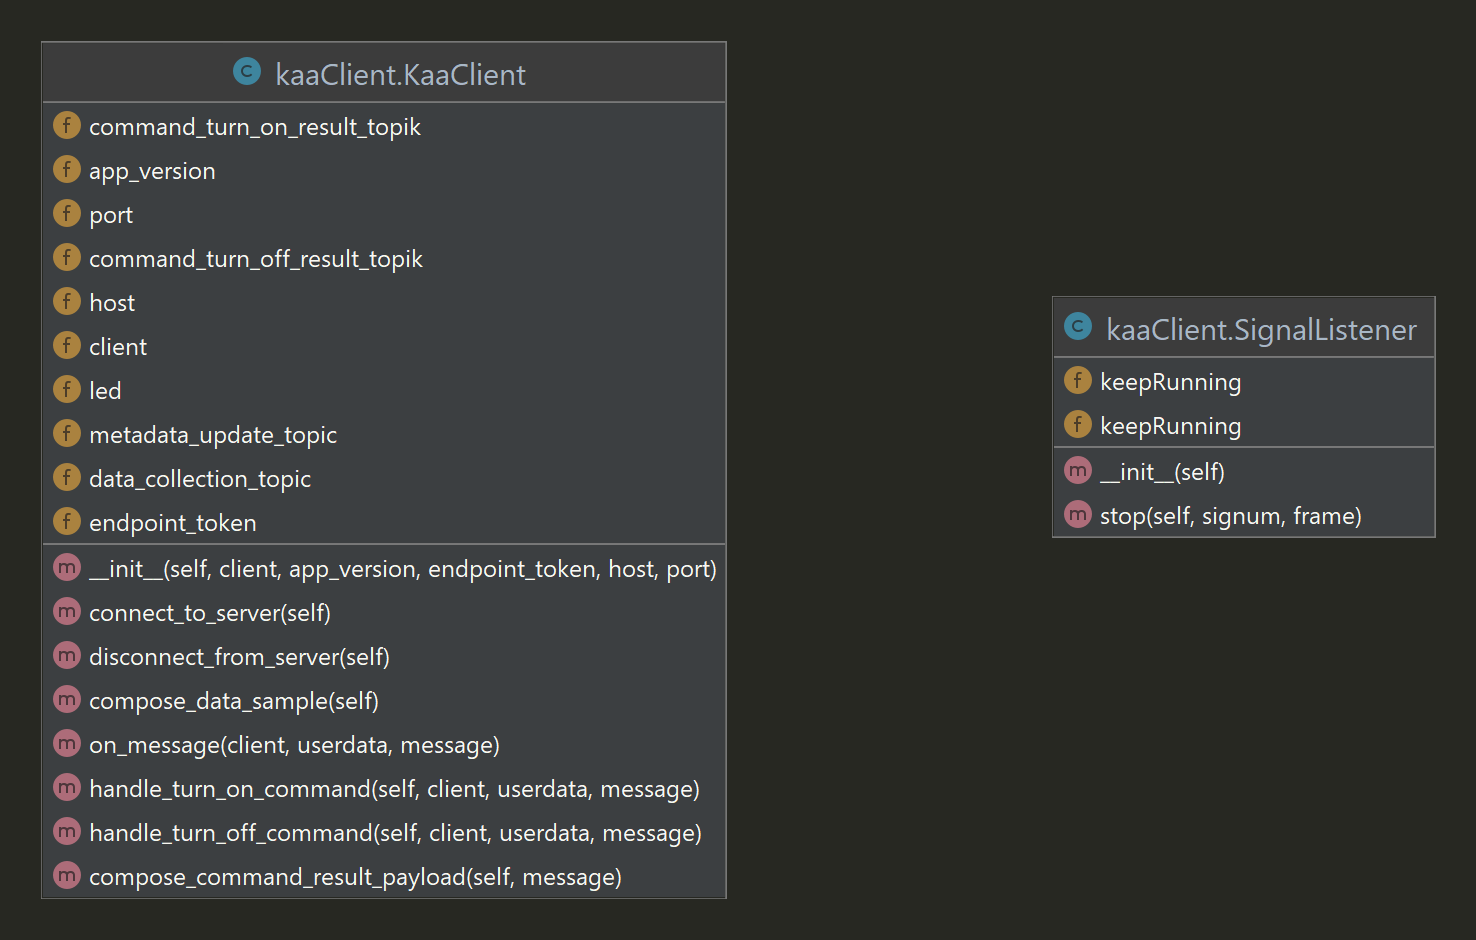
\includegraphics[width=\linewidth]{imagenes/kaaClient.png}
    \caption{Clase de envio de datos de telemetría y ejecución de comandos}
    \label{fig:figure-diseño2}
\end{figure}

La clase \textit{MetadataClient} \ref{fig:figure-diseño1} establece una primera conexión con la aplicación, recoge los datos a nivel hardware de la Raspberry y los envía para actualizar la información en la aplicación. \\

La segunda clase \textit{KaaClient}, hace una conexión con la cual enviamos datos de telemetría, en concreto, obtenemos cada cierto tiempo la temperatura de la CPU de la Raspberry y se envía esta y el momento de tiempo en el que se produce el envio. También incluye funciones para gestionar el encencido y apagado de un led conectado a la Raspberry. \\

El led estará conectado a la Raspberry como se muestra en la figura \ref{fig:figure12}.

\begin{figure}[p]
    \centering
    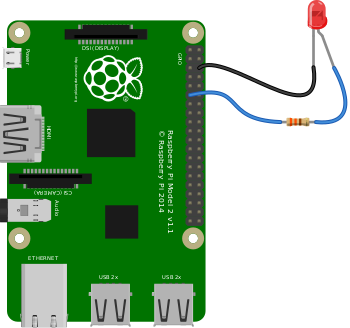
\includegraphics[width=\linewidth]{imagenes/led_bb.png}
    \caption{Conexion del led con Raspberry \cite{raspberry-led}}
    \label{fig:figure12}
\end{figure}

Por último, la clase \textbf{SignalListener} que se usa para poder parar la ejecución de la comunicación desde una E/S. \\

\subsection{Bibliotecas usadas}

\subsubsection{subprocess}

Para obtener los dispositivos conectados a la Raspeberry se usa \textbf{subprocess}. El módulo de subprocesos permite generar nuevos procesos, conectarse a sus tuberías de entrada/salida/error y obtener sus códigos de retorno. \cite{subprocess}

\subsubsection{GPIO Zero}

Una sencilla interfaz para dispositivos GPIO con Raspberry Pi, desarrollada y mantenida por Ben Nuttall y Dave Jones. Se usa para obtener la temperatura de la CPU y para encender/apagar el led de la Raspberry. \cite{gpiozero}

\subsubsection{decouple}

Decouple ayuda a organizar la configuración para que puedas cambiar los parámetros sin tener que volver a desplegar la aplicación. En un fichero .env se almacena los datos sensibles para no mostrarlos al público y se cargan una vez antes de iniciar la comunicación. \cite{decouple}

\subsubsection{paho mqtt}

Como se ha mencionado ya, sirve para establecer la conexión mqtt. \cite{paho-mqtt}

\newpage

\section{Explotación de vulnerabilidad}

Para empezar, ya que vamos a trabajar con MQTT vamos a analizar este protocolo de comunicación para posteriormente atacarlo para así explotar una vulnerabilidad de nuestra aplicación. Una vez visto como funciona MQTT, veremos las etapas de un ataque y las herramientas que necesitamos en cada una de las etapas.

\subsection{Diseño de MQTT}

Ya se habló de este protocolo en \ref{protocolos}. Cada protocolo IoT requiere diferentes vectores de ataque. MQTT no es, por defecto, seguro, y muchos despliegues de MQTT parecen haberse saltado la letra pequeña cuando se trata de usar MQTT de forma segura. Así que vamos a explotarlo. \\

La definición oficial de MQTT viene de \textbf{mqtt.org} \cite{mqtt}: \\

\textit{``MQTT son las siglas de MQ Telemetry Transport. Se trata de un protocolo de publicación/suscripción, extremadamente sencillo y ligero, diseñado para dispositivos limitados y redes de bajo ancho de banda, alta latencia o poco fiables. Los principios de diseño consisten en minimizar el ancho de banda de la red y los requisitos de recursos de los dispositivos, al tiempo que se intenta garantizar la fiabilidad y cierto grado de seguridad en la entrega. Estos principios también hacen que el protocolo sea ideal para el emergente mundo de los dispositivos conectados "máquina a máquina" (M2M) o "Internet de las cosas", y para aplicaciones móviles en las que el ancho de banda y la energía de la batería son muy importantes. ``} \\


MQTT es un protocolo de publicación/suscripción que permite la comunicación de uno a muchos a través de un broker MQTT. Poder comunicarse con todos los dispositivos conectados al broker facilita los ataques activos a gran escala. Un atacante que sea capaz de espiar y saber qué tipo de mensajes se están enviando a través del broker puede utilizar posteriormente esta información para atacar simultáneamente a todos los dispositivos conectados a él. \\

Tiene una característica llamada suscripción con comodines, y muchos usuarios de MQTT pasan por alto las implicaciones de esto en la seguridad. Un despliegue por defecto de MQTT sin autorización permite a cualquier cliente conectado suscribirse a todos los mensajes, y un atacante puede utilizar esta información para conocer y registrar todos los mensajes intercambiados en una solución IoT. Por esto, es bastante factible realizar un ataque de escalado de privilegios. \cite{mqtt-security-1} \\


\subsection{Características de MQTT}

\begin{itemize}
    \item Patrón de publicación y suscripción.
    \item Formatos de paquetes simples: cargas útiles binarias.
    \item Version actual: 3.1.1 (Dec/2015).
    \item El protocolo se ejecuta a través de TCP.
    \item Puerto por defecto: 1883/TCP (no encriptado).
\end{itemize}


El modelo de \textbf{publicación/suscripción} se compone de:

\begin{itemize}
    \item \textbf{Editor,} publica un mensaje en uno (o varios) temas del broker.
    \item \textbf{Broker,} dirige todos los mensajes de los editores a los suscriptores.
    \item \textbf{Tema,} consta de uno o varios niveles separados por una barra diagonal (por ejemplo, /smartshouse/livingroom/temperature).
\end{itemize}

\begin{figure}[hb!]
    \centering
    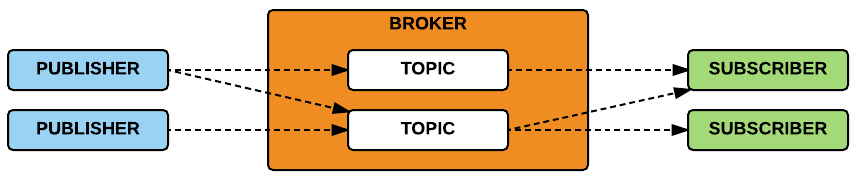
\includegraphics[width=\linewidth]{imagenes/sub-pattern-mqtt.png}
    \caption{Modelo publicación/suscripción \cite{disenio-mqtt}}
    \label{fig:figure13-mqtt-design}
\end{figure}

\subsection{Seguridad en MQTT}

La nota oficial de MQTT acerca de la seguridad de este (\textbf{mqtt.org}) \cite{mqtt}: \\

\textit{``Puedes pasar un nombre de usuario y una contraseña con un paquete MQTT en la V3.1 del protocolo. La encriptación a través de la red puede ser manejada con SSL, independientemente del protocolo MQTT en sí mismo (vale la pena señalar que SSL no es el más ligero de los protocolos, y añade una sobrecarga de red significativa). Se puede añadir seguridad adicional mediante una aplicación que cifre los datos que envía y recibe, pero esto no es algo integrado en el protocolo, con el fin de mantenerlo simple y ligero.``}\\

Aquí tenemos dos puntos a considerar:

\begin{enumerate}
    \item La autenticación es totalmente opcional
    \item Si se realiza la autenticación, el cifrado no se utiliza por defecto (las credenciales se envían en texto claro). Los ataques MITM aún pueden ser ejecutados para robar contraseñas.
\end{enumerate}

\subsection{Fases de un ataque}

Para poder contrarrestar un ataque debemos conocer las fases de este, por esto vamos a hacer un \textbf{test de intrusión} o \textbf{Pentest}. Esto es una prueba de seguridad ofensiva que simula un ataque real en un entorno controlado. El objetivo principal de este tipo de pruebas es identificar las posibles brechas en la seguridad de un sistema de manera que, al simular el comportamiento de los atacantes reales, podamos descubrir vulnerabilidades y agujeros de seguridad que necesiten ser corregidos para que no sean explotados por parte de atacantes reales. \cite{pentesting} \\

Las fases y tecnologías dentro de cada fase que nos encontramos son:

\begin{enumerate}
    \item \textbf{Reconocimiento}, se recolecta información del sistema de forma activa o pasiva. En este caso se van a usar herramientas como nmap o netstat para recopilar información de dominios, IPs, puertos y servicios.
    \item \textbf{Análisis de vulnerabilidades}, aquí se analizará la información recopilada de la fase de reconocimiento. Se puede investigar por internet posibles vulnerabilidad, por ello se puede mencionar a \textbf{CVE} \footnote{https://cve.report/vendor/mqtt}, para conocer posibles vulnerabilidad.
    \item \textbf{Explotación}, en esta fase se realizan las acciones necesarias para poder comprometer al sistema, los usuarios o la información que se maneja. Para este proyecto se usará \textbf{Metasploit}, es una herramienta que proporciona información acerca de vulnerabilidades de seguridad y ayuda en test de penetración.
\end{enumerate}


}